\section{Final results (mode shapes comparison)}
\label{sec:final_results}

Even if the comparison between the experimental FRFs and the numerical FRFs in the complex plane is a good way to validate the identified parameters, it is also useful to compare the mode shapes obtained from the experimental data with the ones obtained from the numerical model.

In the following figures, the experimental (from flexible body theory) and numerical mode shapes are compared for the first 4 modes of the system.
In particular, even if in theory the mode shapes are characteristic of the structure per se, the numerical model is not able to capture exactly the same shape for every set of input-output points.

To be consistent with the previously shown FRF figures, we are now going to represent the experimental mode shapes in blue, and the numerical mode shapes computed considering an input in $x_k = 1.0m$ and an output in $y_j = 0.6m$ is shown.

\begin{figure}[H]
    \begin{minipage}[b]{0.45\textwidth}
        \centering
        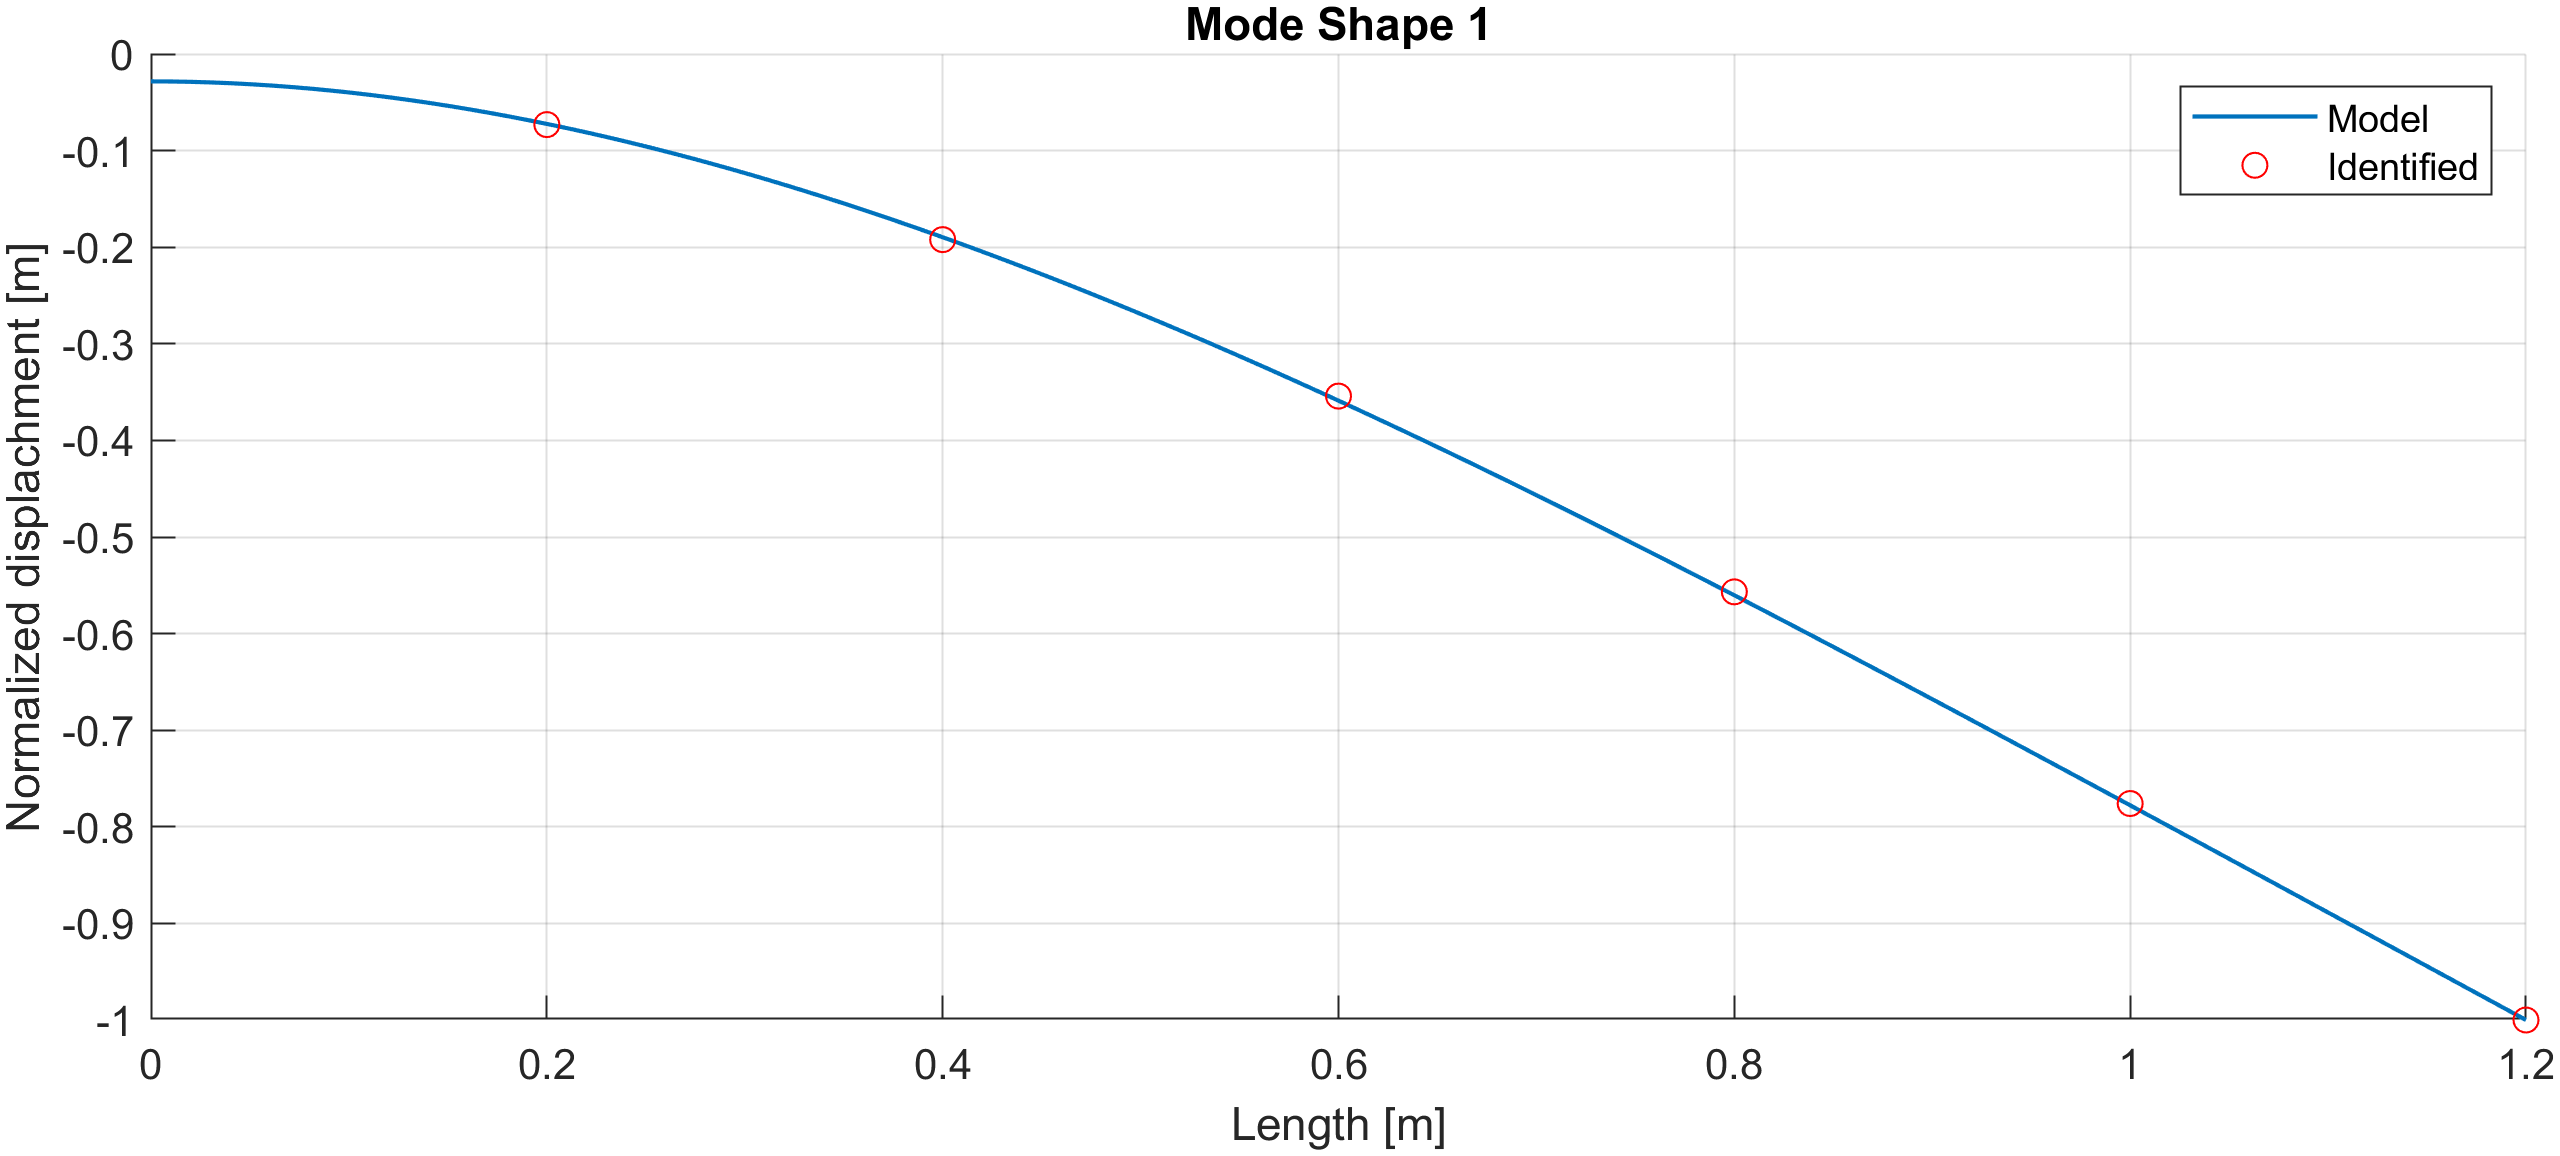
\includegraphics[width=\textwidth]{img/MATLAB/Part_A/Comparison_ModeShape_01.png}
    \end{minipage}
    \hfill
    \begin{minipage}[b]{0.45\textwidth}
        \centering
        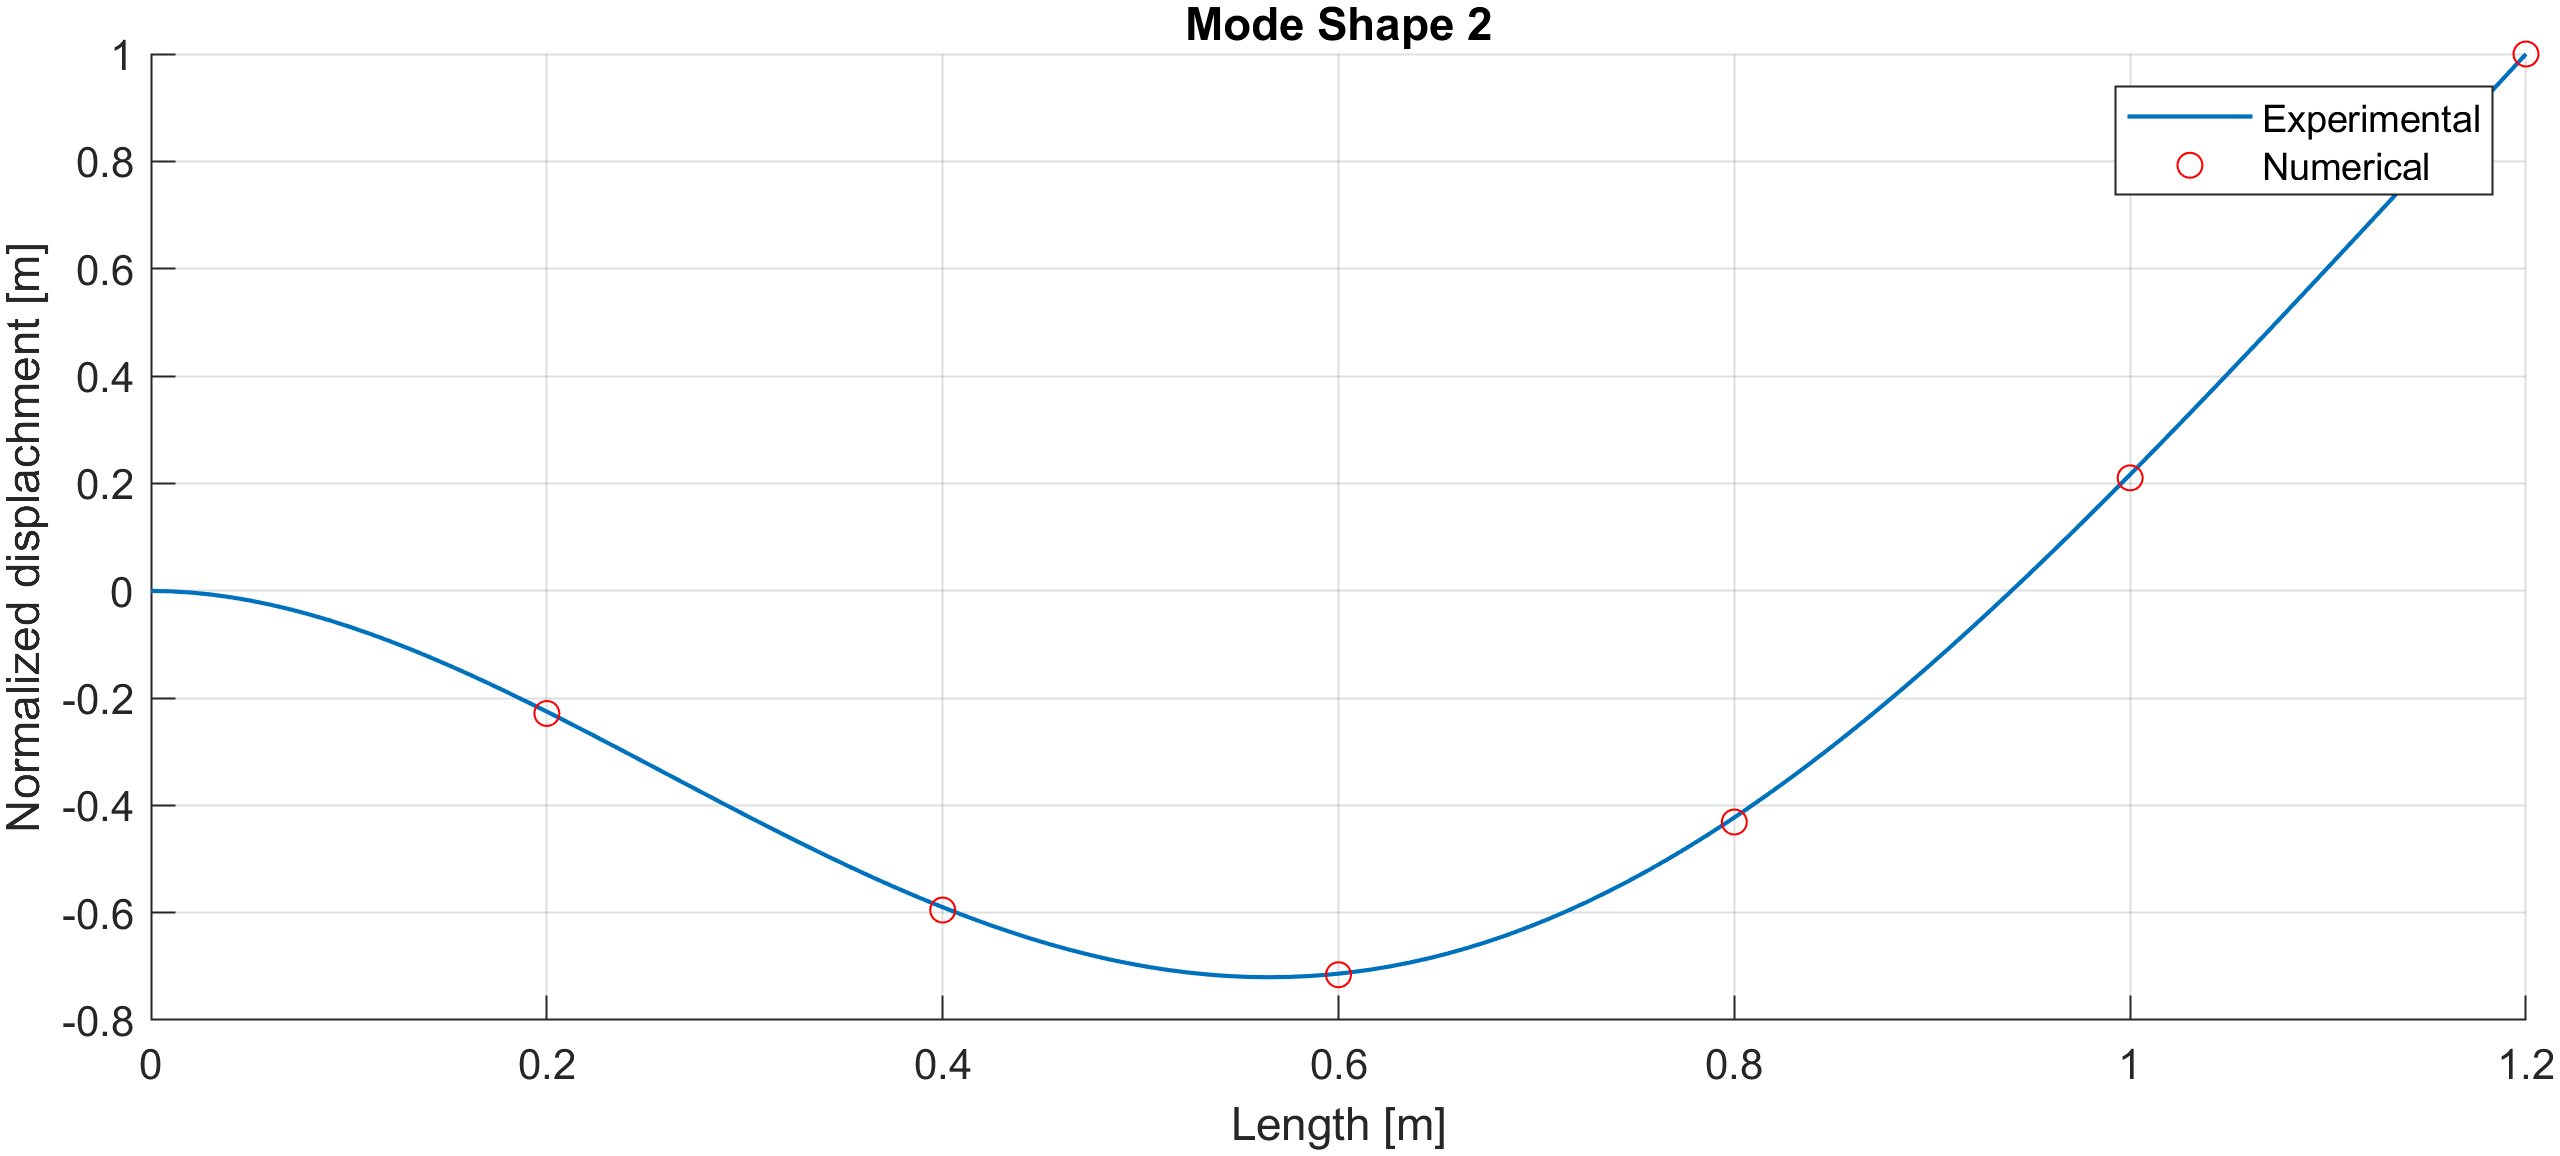
\includegraphics[width=\textwidth]{img/MATLAB/Part_A/Comparison_ModeShape_02.png}
    \end{minipage}
    \begin{minipage}[b]{0.45\textwidth}
        \centering
        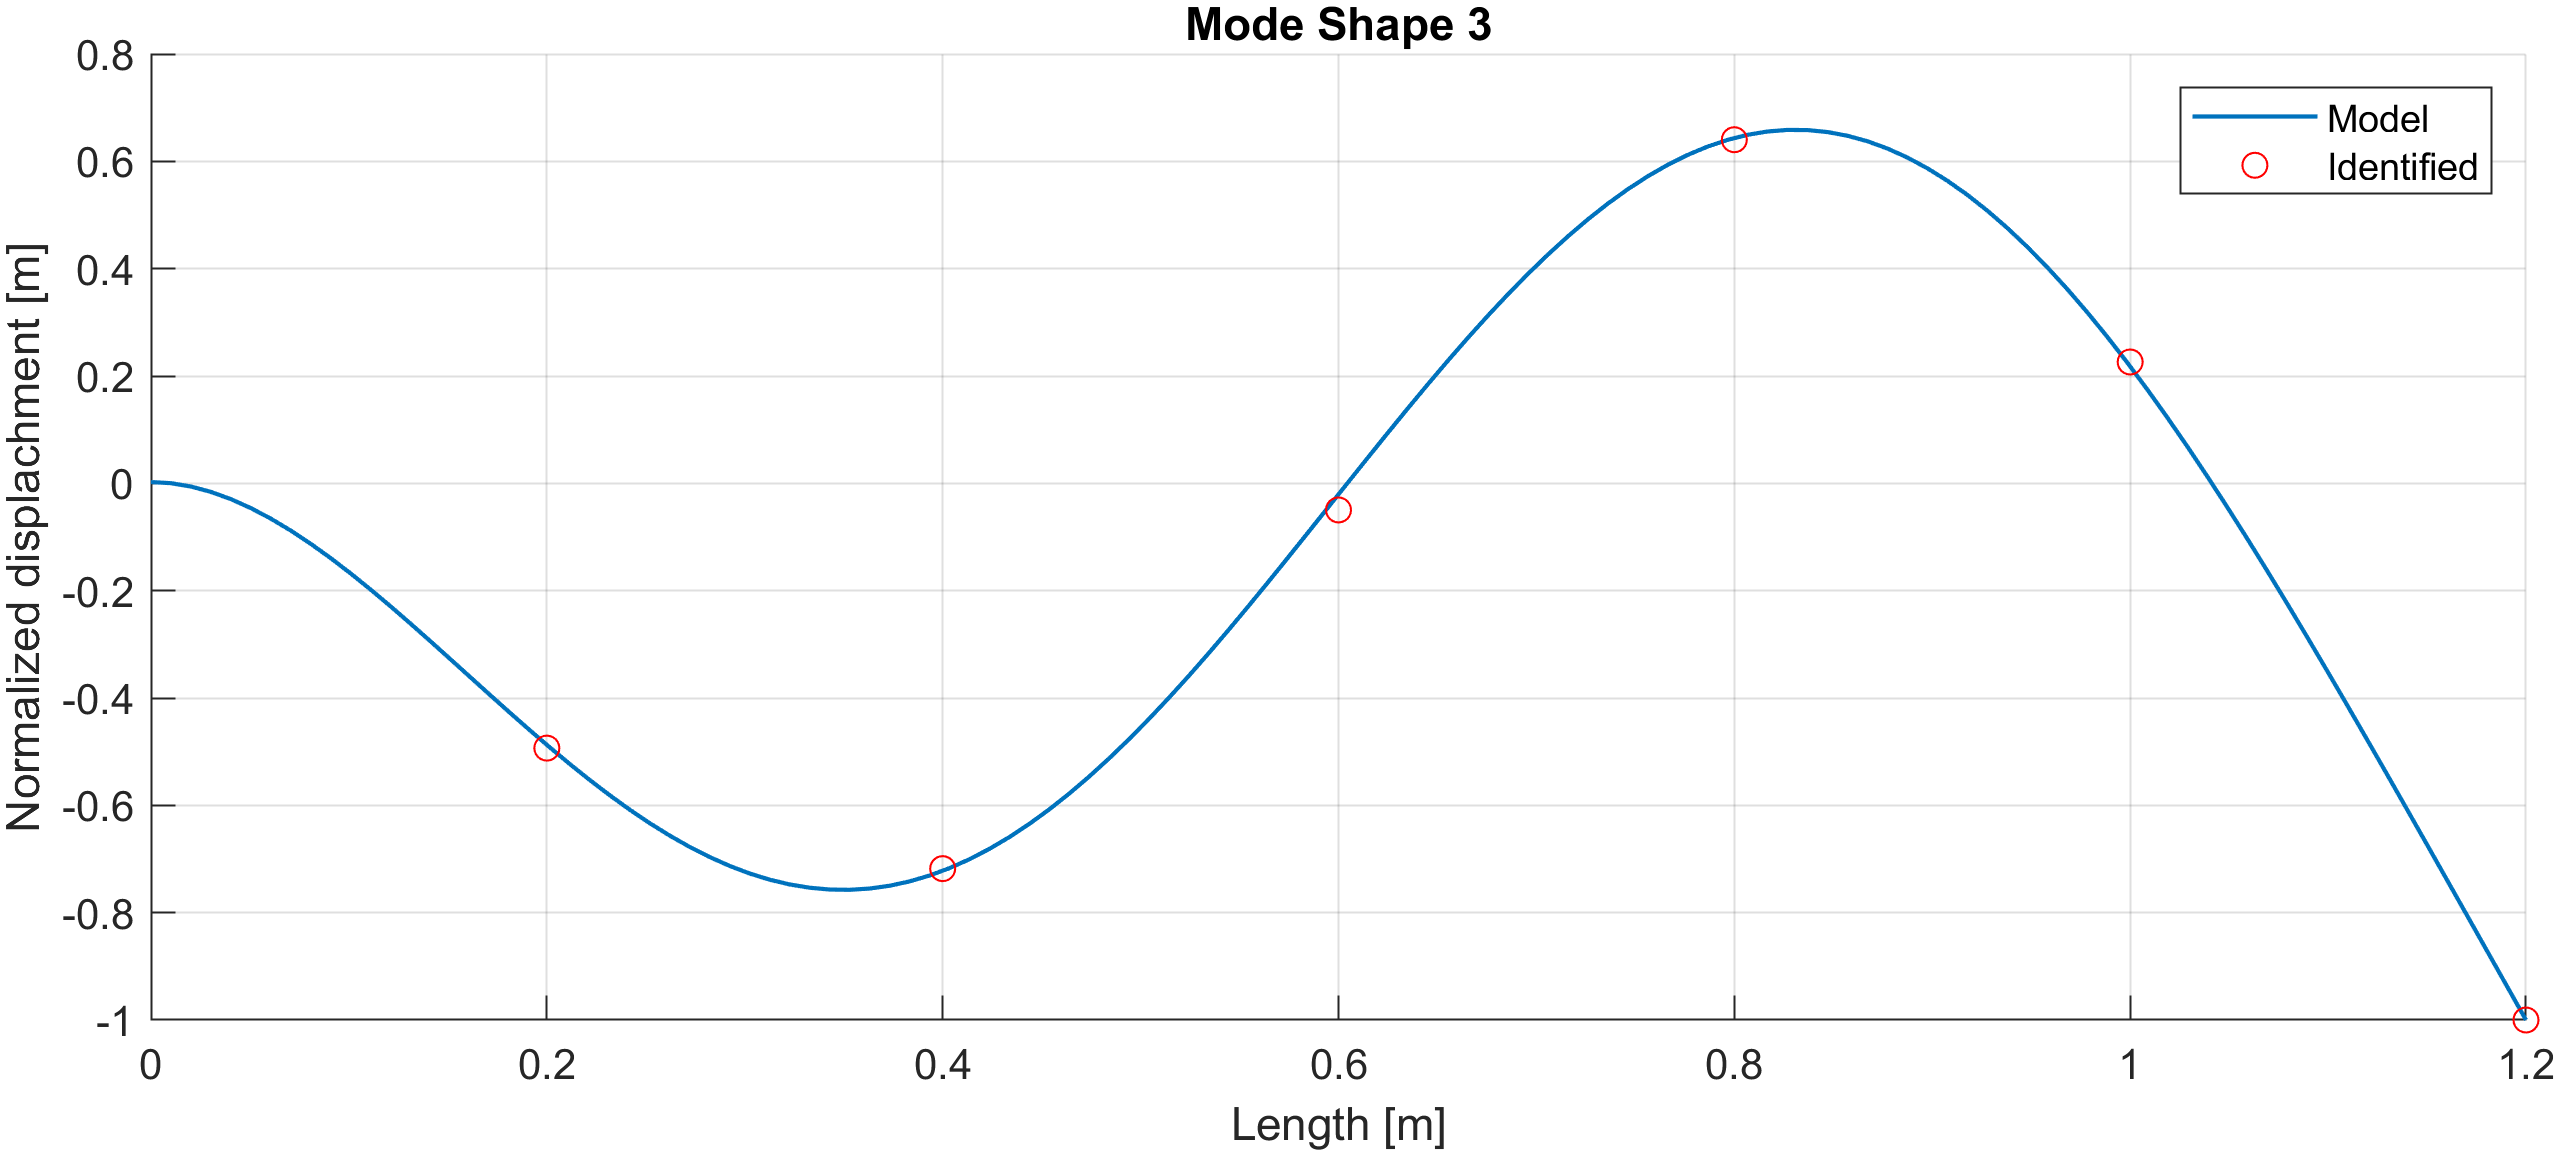
\includegraphics[width=\textwidth]{img/MATLAB/Part_A/Comparison_ModeShape_03.png}
    \end{minipage}
    \hfill
    \begin{minipage}[b]{0.45\textwidth}
        \centering
        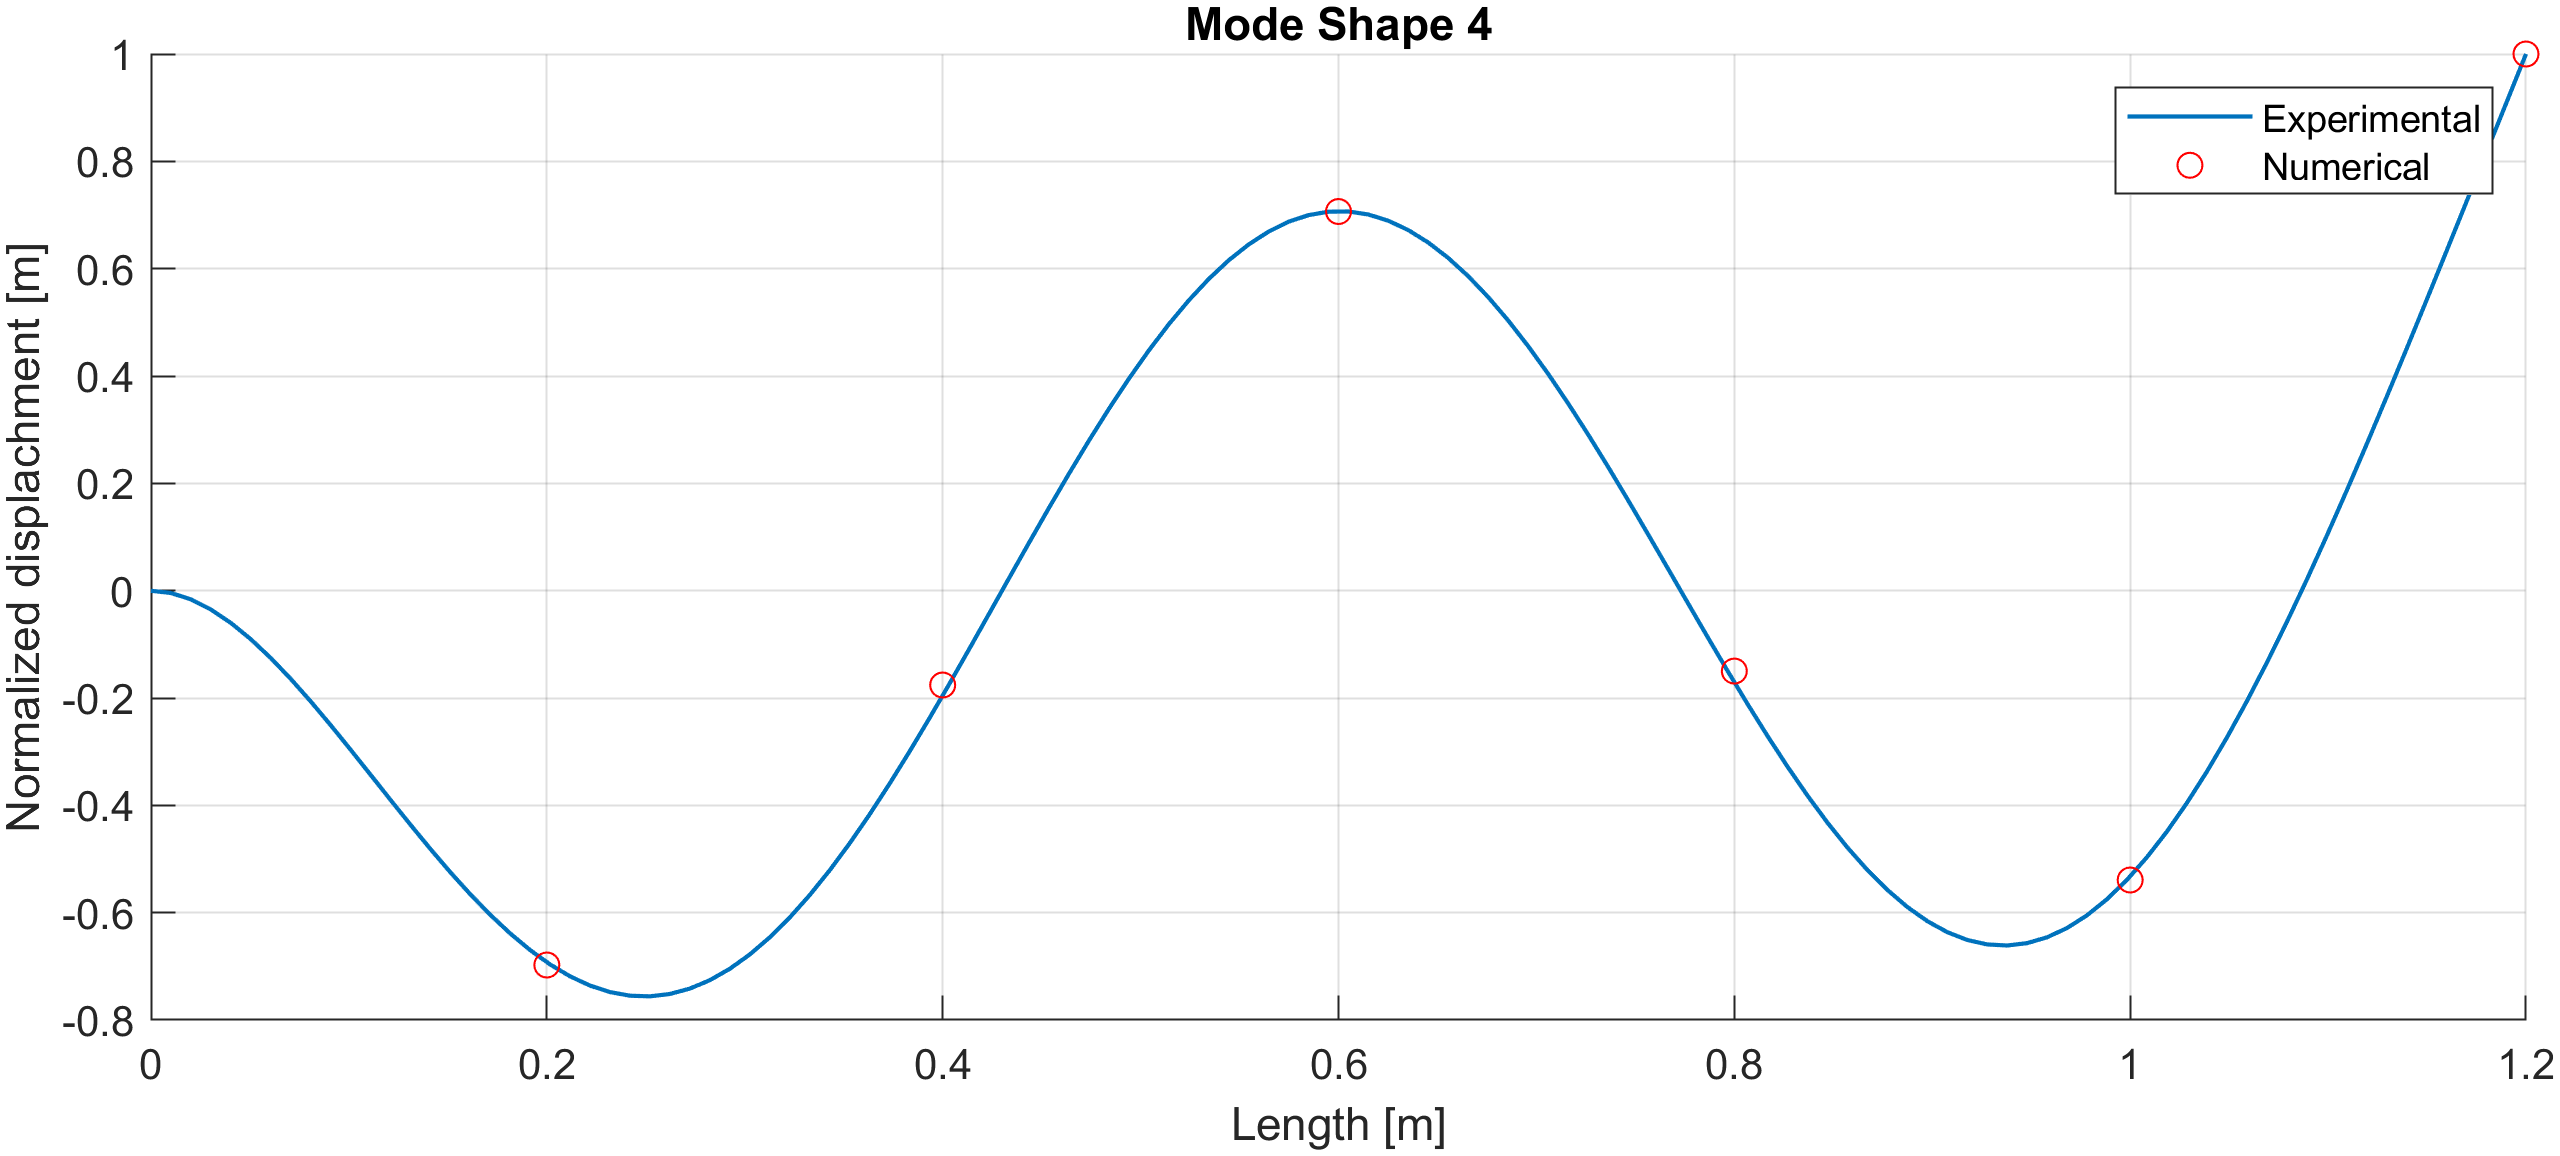
\includegraphics[width=\textwidth]{img/MATLAB/Part_A/Comparison_ModeShape_04.png}
    \end{minipage}
    \caption{Comparison between experimental and numerical mode shapes}
    \label{fig:Mode_shapes_comparison}
\end{figure}

Numerically speaking, we can also report the relative error between the experimental and numerical mode shapes, computed as:

\begin{equation}
    \text{Relative error} = \frac{\sum_{i=1}^{N} \left| \phi_{\text{exp},i} - \phi_{\text{num},i} \right|}{\sum_{i=1}^{N} \left| \phi_{\text{exp},i} \right|}
\end{equation}

Where $\phi_{\text{exp},i}$ and $\phi_{\text{num},i}$ are the $i$-th components of the experimental and numerical mode shapes, respectively.

The relative error for the first 4 modes of the system is reported in the following table.

\begin{center}
    \huge{Table values to be replaced with the correct ones.}
\end{center}

\begin{table}[H]
    \centering
    \begin{tabular}{lccc}
        \hline
        Mode & Experimental & Numerical & Relative error \\
        \hline
        1    & Experimental & Numerical & Relative error \\
        2    & Experimental & Numerical & Relative error \\
        3    & Experimental & Numerical & Relative error \\
        4    & Experimental & Numerical & Relative error \\
        \hline
    \end{tabular}
    \caption{Relative error between experimental and numerical mode shapes}
    \label{tab:Relative_error_mode_shapes}
\end{table}
